\documentclass{article}
\usepackage[utf8]{inputenc}

\usepackage{graphicx}
\usepackage{indentfirst}
\usepackage{hyperref}

\setlength{\parskip}{6pt}

\title{True Sight - Manual}
\author{Ewan "Binary" Barel}
\date{12 August 2022}

\begin{document}

\maketitle

\tableofcontents

\newpage

\section{Introduction}

True Sight is a Burp Suite extension designed to provide auditors with collaborative documentation capabilities. This manual aims to describe the life cycle of the extension and review its features in-depth.

\section{Build}

This extension uses the \href{https://gradle.com}{Gradle} build system and comes with the Gradle wrapper. This way, apart from having a \href{https://www.oracle.com/java/technologies/downloads/}{Java Development Kit} version 8 or later installed, nothing else is required to produce the extension's JAR file.

In order to initiate the building process, run the following command from the root of the repository: \verb|gradlew shadowJar|

Once the building process completes, the JAR file will be located under the following directory: \verb|build/libs/truesight-all.jar|

\section{Projects}

Burp Suite premium versions already provide a way to save and load projects. However, True Sight uses a completely separate way of handling projects which makes it completely free to use on any version. (Moreover, the extender API does not provide any ways to interact with this feature.)

Just like Burp Suite, True Sight can run either on temporary or persistent projects:
\begin{itemize}
    \item A temporary project cannot be written to the disk and its contents will be lost once it unloads (either by loading another project or by unloading the extension) with no way of recovering.
    \item A persistent project can be loaded and unloaded at any time and its data is saved automatically, on behalf of the user.
\end{itemize}

A True Sight persistent project takes the form of a directory which can be tracked by a \href{https://en.wikipedia.org/wiki/Version_control}{version control system} for sharing and collaborating. It is loaded from the "Settings" tab of the extension (section \ref{settings project}) and contains a few files which will be explained in their appropriate sections:
\begin{itemize}
    \item \verb|catalog|: directory containing the documents of the catalog (section \ref{catalog}).
    \item \verb|workflows|: directory containing the workflows (section \ref{workflows}).
    \item \verb|substitutions.json|: file containing the project scope variable name substitutions.
\end{itemize}

\section{Settings}

This section will cover the settings of the extension which can be changed from the extension's sub-tab of the same name.

\begin{figure}[h]
    \centering
    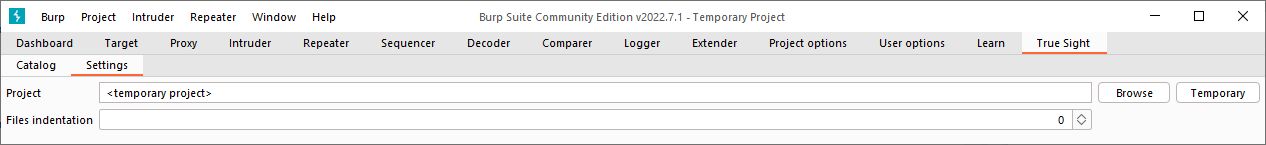
\includegraphics[width=\textwidth]{assets/settings.png}
    \caption{The settings tab}
    \label{fig:settings}
\end{figure}

\subsection{Project} \label{settings project}

The "Project" setting is a pathname to the root directory of a persistent True Sight project. The extension remembers it between loads. In the case of a temporary project the indication \verb|<temporary project>| will take place of the pathname.

The "Browse" and "Temporary" buttons respectively load persistent and temporary projects, and have the side-effect of unloading the previously loaded project.

When the "Browse" button is clicked, a file explorer appears and the user is expected to open the root directory of a persistent project. In order to load a new empty persistent project, the user has to create and open an empty directory.

When the "Temporary" button is clicked, the currently loaded project unloads and a new empty temporary project takes its place.

\subsection{Files indentation}

The "Files indentation" setting is a number defining how many spaces are used for indenting the JSON files of a persistent project. The extension remembers it between loads. This is an extension setting, not a project setting, meaning it is shared across all projects that gets loaded and unloaded during the extension's lifetime.

Changing this setting will not affect all of the project files right away. In fact, because True Sight only writes to disk what needs to be saved, changing this setting will only take effect on files solicited after the change. In other words, the files will not have their indentation updated unless they are written to again by the extension.

It is recommended to keep the indentation level to 0 for smaller file sizes.

\section{Documents}

The primary feature of True Sight is the documentation of HTTP messages. This is achieved by creating documents which are covered in this section.

\subsection{Overview}

A document, in True Sight terminology, is a full copy of an HTTP message's request and response along with additional fields to store documentation-related information. 

A document is distinguished by its \href{https://en.wikipedia.org/wiki/Universally_unique_identifier}{unique identifier} and can be given a title, notes, and highlighted with any color. The user can also take notes of about any of a document's request or response fields as well as applying name substitutions. Finally, documents that are related in some way can be brought together into workflows (section \ref{workflows}).

All of these elements can be edited in the document editor and are saved automatically on behalf of the user when it closes. There can be as many editors open at the same time but only one per document.

\begin{figure}[h]
    \centering
    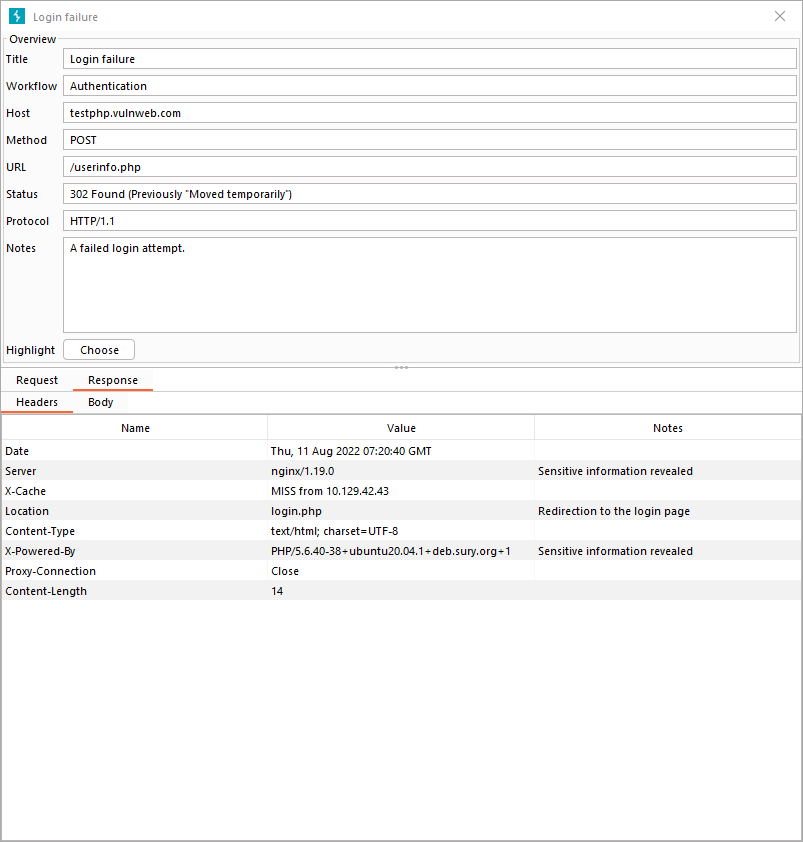
\includegraphics[width=0.75\linewidth]{assets/document_editor.png}
    \caption{A document editor}
    \label{fig:document editor}
\end{figure}

\subsection{Variables}

\subsubsection{Name substitutions}

Any of a document's variable - such as headers, query parameters, cookies or form data fields - can have their name substituted with another either locally (document scope) or globally (project scope).

A local substitution changes the name of a variable in the document whereas a global substitution will apply to any variable of the same kind and same name. Local substitutions always take precedence over global substitutions. In the case of a persistent project, the global substitutions are stored as a JSON file named \verb|substitutions.json| under the root of project.

To set a location substitution: double click on the name field of a variable and type in its new substitute. To set a global substitution, select one or more variables, right click and choose "Apply global substitution": a dialog will appear prompting you to enter the global substitution to set. 

To undo a substitution, give it an empty name or the original variable's name. The original name of a variable can be viewed by hovering its name field.

\subsubsection{Copying to the clipboard}

Variables can be copied to the clipboard in their original format by selecting one or more, right-clicking and choosing "Copy to clipboard". In this case the substitutions are not applied and the original variable names are used for convenience.

\section{Catalog} \label{catalog}

The catalog is the main component of a True Sight project. It is the place where all the documents of a project are gathered. This section will cover how to use it and how to convert HTTP messages into documents. 

\subsection{Overview}

The catalog appears as a table in its own sub-tab. It is very similar to the HTTP history sub-tab of Burp Suite's Proxy tab, except that each row corresponds to a specific document and there are fewer columns.

In the case of a persistent project, the catalog possesses its own directory named \verb|catalog| under the project's root. Each of the documents it stores is saved under this directory as a JSON file with the document's unique identifier as its filename.

\begin{figure}[h]
    \centering
    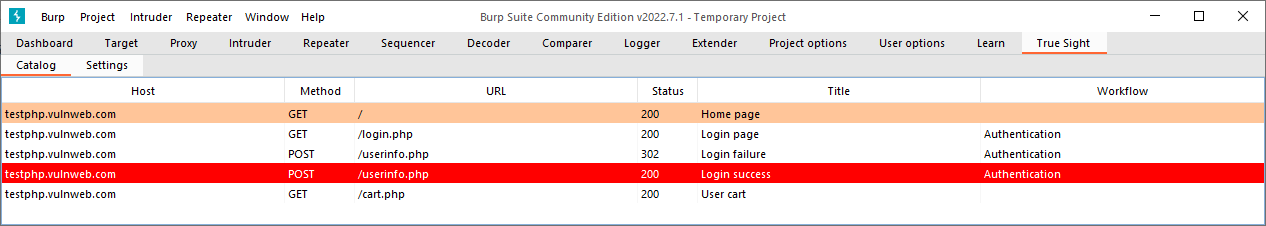
\includegraphics[width=\textwidth]{assets/catalog.png}
    \caption{The catalog tab}
    \label{fig:catalog}
\end{figure}

\subsection{Creating documents from HTTP messages}

A document is created and stored in the catalog by right-clicking inside of a Burp Suite message editor or by selecting messages from the HTTP history sub-tab of Burp Suite's Proxy tab, right-clicking and choosing "Extensions", "True Sight", "Send to Catalog". Every selected message must have a response for the context menu action to show up. 

When sending messages from the HTTP history to the catalog, True Sight will copy the message's comment and highlight respectively into the new document's title and highlight fields. Furthermore, if a message has identical contents with a document in the catalog, it is automatically rejected to avoid creating duplicates.

\begin{figure}[h]
    \centering
    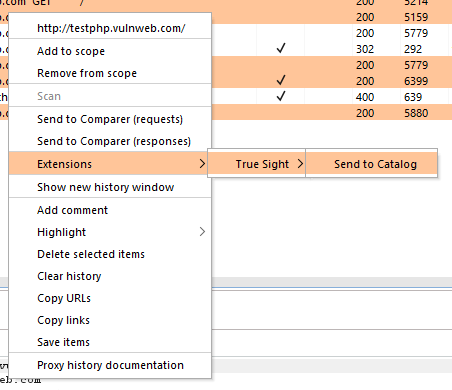
\includegraphics[width=0.5\linewidth]{assets/ctxmenu.png}
    \caption{Sending HTTP messages to the catalog}
    \label{fig:ctxmenu}
\end{figure}

\subsection{Interactions with documents}

Some document fields can be changed directly from within the catalog:
\begin{itemize}
    \item The title and workflow of a document can be changed by double left-clicking on the corresponding column.
    \item The highlight of many documents can be set at once by selecting one or more, right-clicking and choosing "Highlight". 
    \item The workflow of many documents can be changed at once by selecting more than one document, right-clicking and choosing "Workflow".
\end{itemize}

Documents can be deleted from the catalog by selecting one or more, right-clicking and choosing "Delete" or using the \verb|Delete| or \verb|Backspace| keystroke shortcut.

Finally, the HTTP requests contained in a document can be sent to Burp Suite's repeater by selecting one or more, right-clicking and choosing "Send to Repeater" or using the \verb|Ctrl+R| keystroke shortcut.

\section{Workflows} \label{workflows}

A workflow is an ordered set of documents which describes a flow of HTTP messages. It is distinguished by a unique identifier and a name. The user can provide additional information about a workflow in a dedicated description field and re-organize the order of the documents to properly reflect the flow of the messages.

In the case of a persistent project, workflows possess their own directory named \verb|workflows| under the project's root. Each of them is saved under this directory as a JSON file with their unique identifier as the filename.

To edit a workflow, select from the catalog one of the documents that is assigned to the workflow to be opened, right-click and choose "Workflow". There can be as many editors open at the same time but only one per workflow. 

Inside of a workflow editor, the name and description can be changed and documents can be re-ordered. However, a name change will fail if any other workflow has the same name (case-insensitive).

To reorder documents, select one, right-click and choose either "Move up" or "Move down". Shortcut keystrokes can also be used: \verb|Shift+Up| or \verb|Ctrl+Y| to move up, and \verb|Shift+Down| or \verb|Ctrl+E| to move down.

A document can be removed from a workflow either by setting its name to an empty one from the catalog, or by selecting it from the workflow editor, right-clicking and choosing "Remove" (which will only affect the workflow unlike "Delete").

Other than that, apart from choosing multiple documents at once and changing their workflow, anything that can be done in the catalog can be done in the workflow editor, and any changes made to a workflow is automatically saved once the latter closes.

\begin{figure}[h]
    \centering
    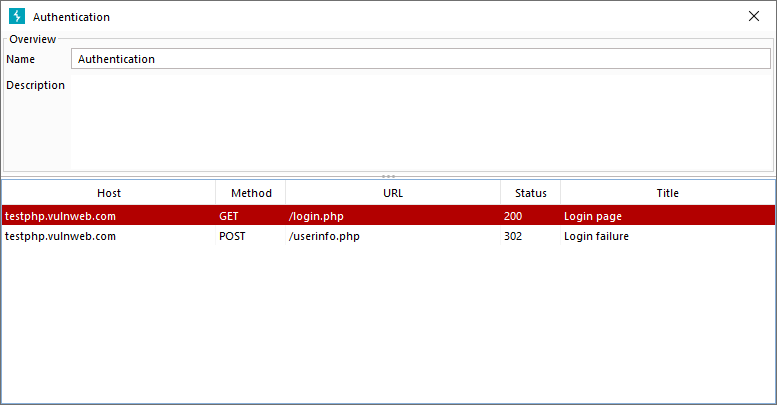
\includegraphics[width=\linewidth]{assets/workflow_editor.png}
    \caption{A workflow editor}
    \label{fig:workflow editor}
\end{figure}

\end{document}
